%%%%%%%%%%%%%%%%%%%%%%%%%%%%%%%%%%%%%%%%%%%%%%%%%%%%%%%%%%%%%%%%%%%%%%%%%%%
%%%%%%%%		 Proyecto Fin de Carrera		   %%%%%%%%
%%%%%%%%	       Presentación de diapositivas		   %%%%%%%%
%%%%%%%%%%%%%%%%%%%%%%%%%%%%%%%%%%%%%%%%%%%%%%%%%%%%%%%%%%%%%%%%%%%%%%%%%%%

\documentclass[utf8, compress]			{beamer}

%%%%%%%%%%%%%%%%%%%%%%%%%        Preámbulo        %%%%%%%%%%%%%%%%%%%%%%%%%

%---------------------------------beamer----------------------------------%

\mode<presentation>
{
    \useinnertheme{rounded}
    \useoutertheme[subsection=true]{miniframes}
    \useoutertheme{split}
    \useoutertheme{shadow}
    \setbeamertemplate{headline}[miniframes theme]{}
    \defbeamertemplate{footline}{pfc slides footline}{
	\leavevmode %
	\hbox{\begin{beamercolorbox} %
	    [wd		= .58\paperwidth, %
	     ht		= 2.5ex, %
	     dp		= 1.125ex, %
	     leftskip	= .3cm plus1fill, %
	     rightskip	= .3cm]{author in head/foot} %
	    \usebeamerfont{author in head/foot}\insertshorttitle
	  \end{beamercolorbox} %
	  \begin{beamercolorbox} %
	    [wd		= .38\paperwidth, %
	     ht		= 2.5ex, %
	     dp		= 1.125ex, %
	     leftskip	= .3cm, %
	     rightskip	= .3cm plus1fil]{title in head/foot} %
	    \usebeamerfont{title in head/foot}\insertshortinstitute
	  \end{beamercolorbox}} %
    	\vskip0pt %
    }
    \setbeamertemplate{footline}[pfc slides footline]{}
    \setbeamertemplate{frametitle}[shadow theme]{}
    \setbeamertemplate{itemize items}[circle]{}
    \setbeamertemplate{enumerate items}[circle]{}
    \setbeamertemplate{sections/subsections in toc}[circle]{}
    \setbeamertemplate{title page}{
	\vbox{}
	\vfill
	\begin{center}
	    \begin{beamercolorbox}[sep=8pt,center]{institute}
		\usebeamerfont{author}\insertinstitute
	    \end{beamercolorbox}
	    \inserttitlegraphic
	    \vskip.4em\par
	    \begin{beamercolorbox}[sep=8pt,center,rounded=true]{title}
		\usebeamerfont{title}\inserttitle
	    \end{beamercolorbox}
	    \vskip.4em\par
	    \begin{beamercolorbox}[sep=8pt,center]{date}
		\usebeamerfont{date}\insertdate
	    \end{beamercolorbox}
	    \begin{beamercolorbox}[sep=8pt,right]{author}
		\usebeamerfont{institute}\insertauthor
	    \end{beamercolorbox}
	\end{center}
	\vfill
    }
    \usecolortheme{orchid}
    \usecolortheme{whale}
}

%--------------------------------\beamer----------------------------------%

\usepackage[spanish]					{babel}
\usepackage[T1]						{fontenc}
\usepackage[altbullet, nofontinfo]			{lucidabr}
\usepackage						{graphicx}
\usepackage{array, booktabs}

\graphicspath{{./pictures/}{../pictures/}}			% graphics

\title[ENDUS: Sistema de medida y aplicación en palmeras in vivo.]{
    Desarrollo de sistema de medida por ultrasonidos de baja frecuencia. \\
    Aplicación al análisis de palmeras in vivo.
}

\newlength{\director}
\settowidth\director{\usebeamerfont{institute}DIRECTOR: Alberto Rodríguez
    Martínez}

\author[José Ramón Gisbert Valls]{
    \vbox{
	\makebox[\director][r]{AUTOR: José Ramón Gisbert Valls}
	\makebox[\director][r]{DIRECTOR: Alberto Rodríguez Martínez}
    }
}

\institute[Universidad Miguel Hernández de Elche]{
    Universidad Miguel Hernández de Elche \medskip\par
    Escuela Politécnica Superior de Elche
}

\date[Septiembre --- 2011]{
    Proyecto Fin de Carrera \\
    Septiembre --- 2011
}

\titlegraphic{
    
\includegraphics[bb = 0 524 152 678, clip, height = 1.4cm,
	keepaspectratio]{logo.pdf}
}

\logo{
    
\includegraphics[bb = 0 524 152 678, clip, height = .8cm,
	keepaspectratio]{logo.pdf}
}

% Convenios tipográficos: siglas (primera vez), siglas, funciones,
% argumentos, propiedades, atributos de propiedades, nombres de canal o
% puerto
\newcommand\psig[1]{\emph{\MakeTextUppercase{#1}}}
\newcommand\sig [1]{\textsc{\MakeTextLowercase{#1}}}
\newcommand\func[1]{\texttt{#1}}
\newcommand\argu[1]{\texttt{#1}}
\newcommand\prop[1]{\textsf{#1}}
\newcommand\atr [1]{\textsf{#1}}
\newcommand\can [1]{\sig{#1}}

% Palabras predefinidas
\newcommand\matlab{\sig{MATLAB}}
\newcommand\kpci  {\sig{KPCI}-3108}
\newcommand\datx  {\sig{DAT}}
\newcommand\gui   {\sig{GUI}}
\newcommand\guide {\sig{GUIDE}}
\newcommand\pc    {\sig{pc}}
\newcommand\ram   {\sig{ram}}
\newcommand\AOUA  {\ensuremath{\mu}\sig{a}741}
\newcommand\kms   {kmus/s}

%%%%%%%%%%%%%%%%%%%%%%%%         Contenido         %%%%%%%%%%%%%%%%%%%%%%%%

\begin{document}


\frame[plain]{\titlepage}

\begin{frame}{Índice}
    \tableofcontents
\end{frame}

\begin{frame}{Objetivos}
    \begin{itemize}
	\item Desarrollo un sistema de medida por ultrasonidos:
	    \begin{itemize}
		\item Valor numérico instantáneo de la señal.
		\item Media aritmética de las muestras tomadas durante un
		    periodo de 250 ms.
		\item Representación gráfica de la señal.
		\item Representación gráfica del espectro instantáneo de la
		    señal.
	    \end{itemize}
	\item Realización de un estudio preliminar que determine la
	    existencia de una relación entre los parámetros medidos en un
	    ENDUS y las condiciones a las que se encuentra expuesto una
	    palmera.
    \end{itemize}
\end{frame}


\section{Desarrollo del sistema de medida}

\subsection{Subsistema físico}

\begin{frame}{Transductores}
    \begin{table} 
	\centering
	\begin{tabular}{l c c}
	    \toprule
	    & \multicolumn{2}{c}{Valor} \\
	    \cmidrule(r){2-3}
	    \multicolumn{1}{c}{Propiedad} &
	    \multicolumn{1}{c}{Sensor} &
	    \multicolumn{1}{c}{Actuador} \\
	    \midrule
	    SPL & 110 dB & --- \\
	    Sensibilidad & --- & -70 dB \\
	    Potencia máxima & --- & 200
	    mW (rms) \\
	    Resistencia & 30 k$\Omega$
	    & 700 $\Omega$ \\
	    \bottomrule
	\end{tabular}
	\caption{Características de los transductores utilizados.}
	\label{tab:trasnducers}
    \end{table}
\end{frame}

\begin{frame}{Acondicionamiento del sensor}
    \begin{figure}
	\centering
	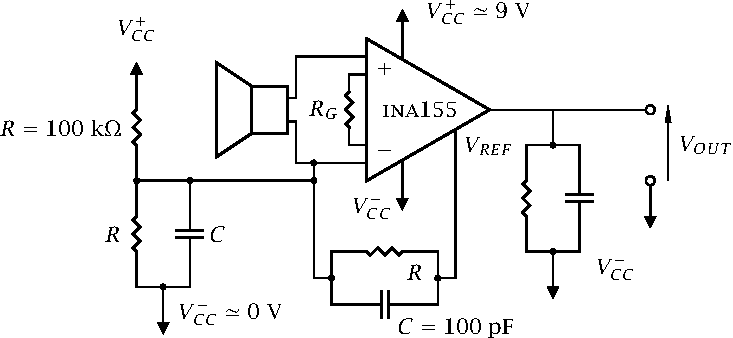
\includegraphics[scale=.5]{sensor.pdf}
	\caption{Única etapa amplificadora formada por un amplificador de
	instrumentación.}
	\label{fig:sensor}
    \end{figure}
\end{frame}

\begin{frame}{Acondicionamiento del actuador}
    \begin{figure}
	\centering
	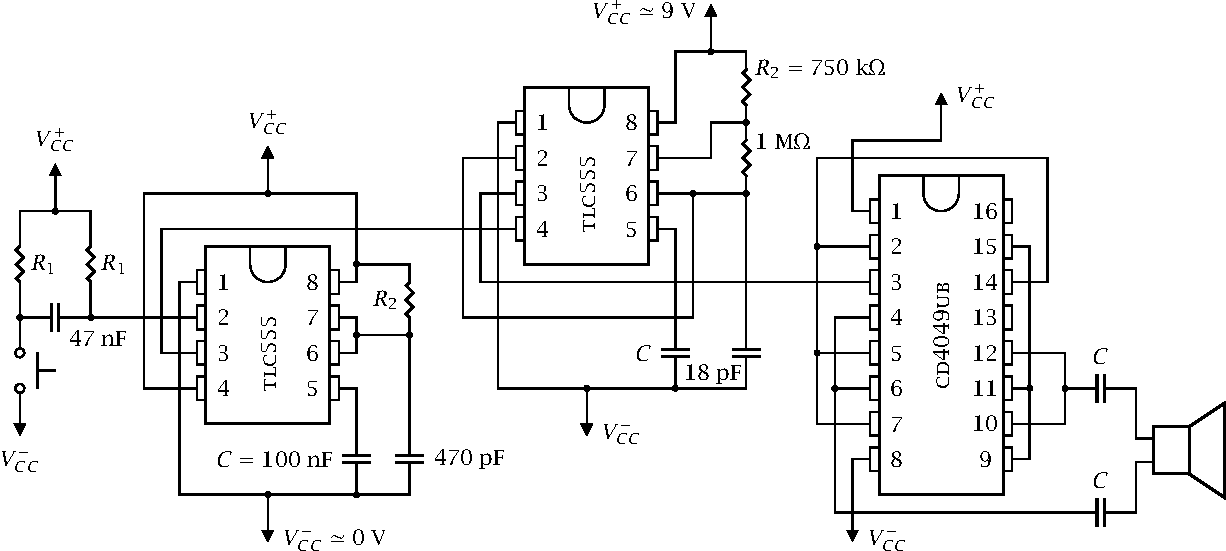
\includegraphics[scale=.5]{actuador.pdf}
	\caption{Tres etapas más una etapa de salida. El circuito genera
	una señal rectangular.}
	\label{fig:actuator}
    \end{figure}
\end{frame}


\subsection{Subsistema de adquisición}

\begin{frame}{Tarjeta de adquisición digital}
    \begin{itemize}
	\item Interfaz PCI (velocidad máxima de transferencia 132 MB/s).
	\item Subsistema de adquisición de señales analógicas.
	\item Subsistema generador de señales analógicas (2 canales de
	    salida analógica).
	\item Subsistema de entrada/salida digital (4 registros de 8 bits
	    de propósito general).
    \end{itemize}
\end{frame}

\begin{frame}{Características de la tarjeta}
    \begin{itemize}
	\item Rendimiento máximo de muestreo de 100 kmus/s.
	\item 16 canales de entrada analógica configurables por software.
	\item Amplificador de instrumentación implementado internamente en
	    la tarjeta, ganancia configurable por software.
	\item Conversor A/D de 16 bits de precisión.
	\item Cola de muestreo de 256 posiciones.
	\item Buffer FIFO con capacidad para 2048 muestras.
    \end{itemize}
\end{frame}

\begin{frame}{Caja de conexiones}
    \begin{itemize}
	\item Necesidad de una interfaz para la realización de las pruebas.
	\item Diseño y construcción de una caja de conexiones.
	    \begin{itemize}
		\item Se parte de dos cables para la interconexión de
		    dispositivos con conectores macho mini-D.
		\item Se retira la cubierta protectora externa y se revelan
		    los hilos de cobre que forman cada cable
		\item Prueba e identificación de los terminales con los
		    cables.
		\item Realización de un mapa de colores.
		\item Construcción de la caja.
	    \end{itemize}
    \end{itemize}
\end{frame}

\newlength{\exterior}
\settoheight\exterior{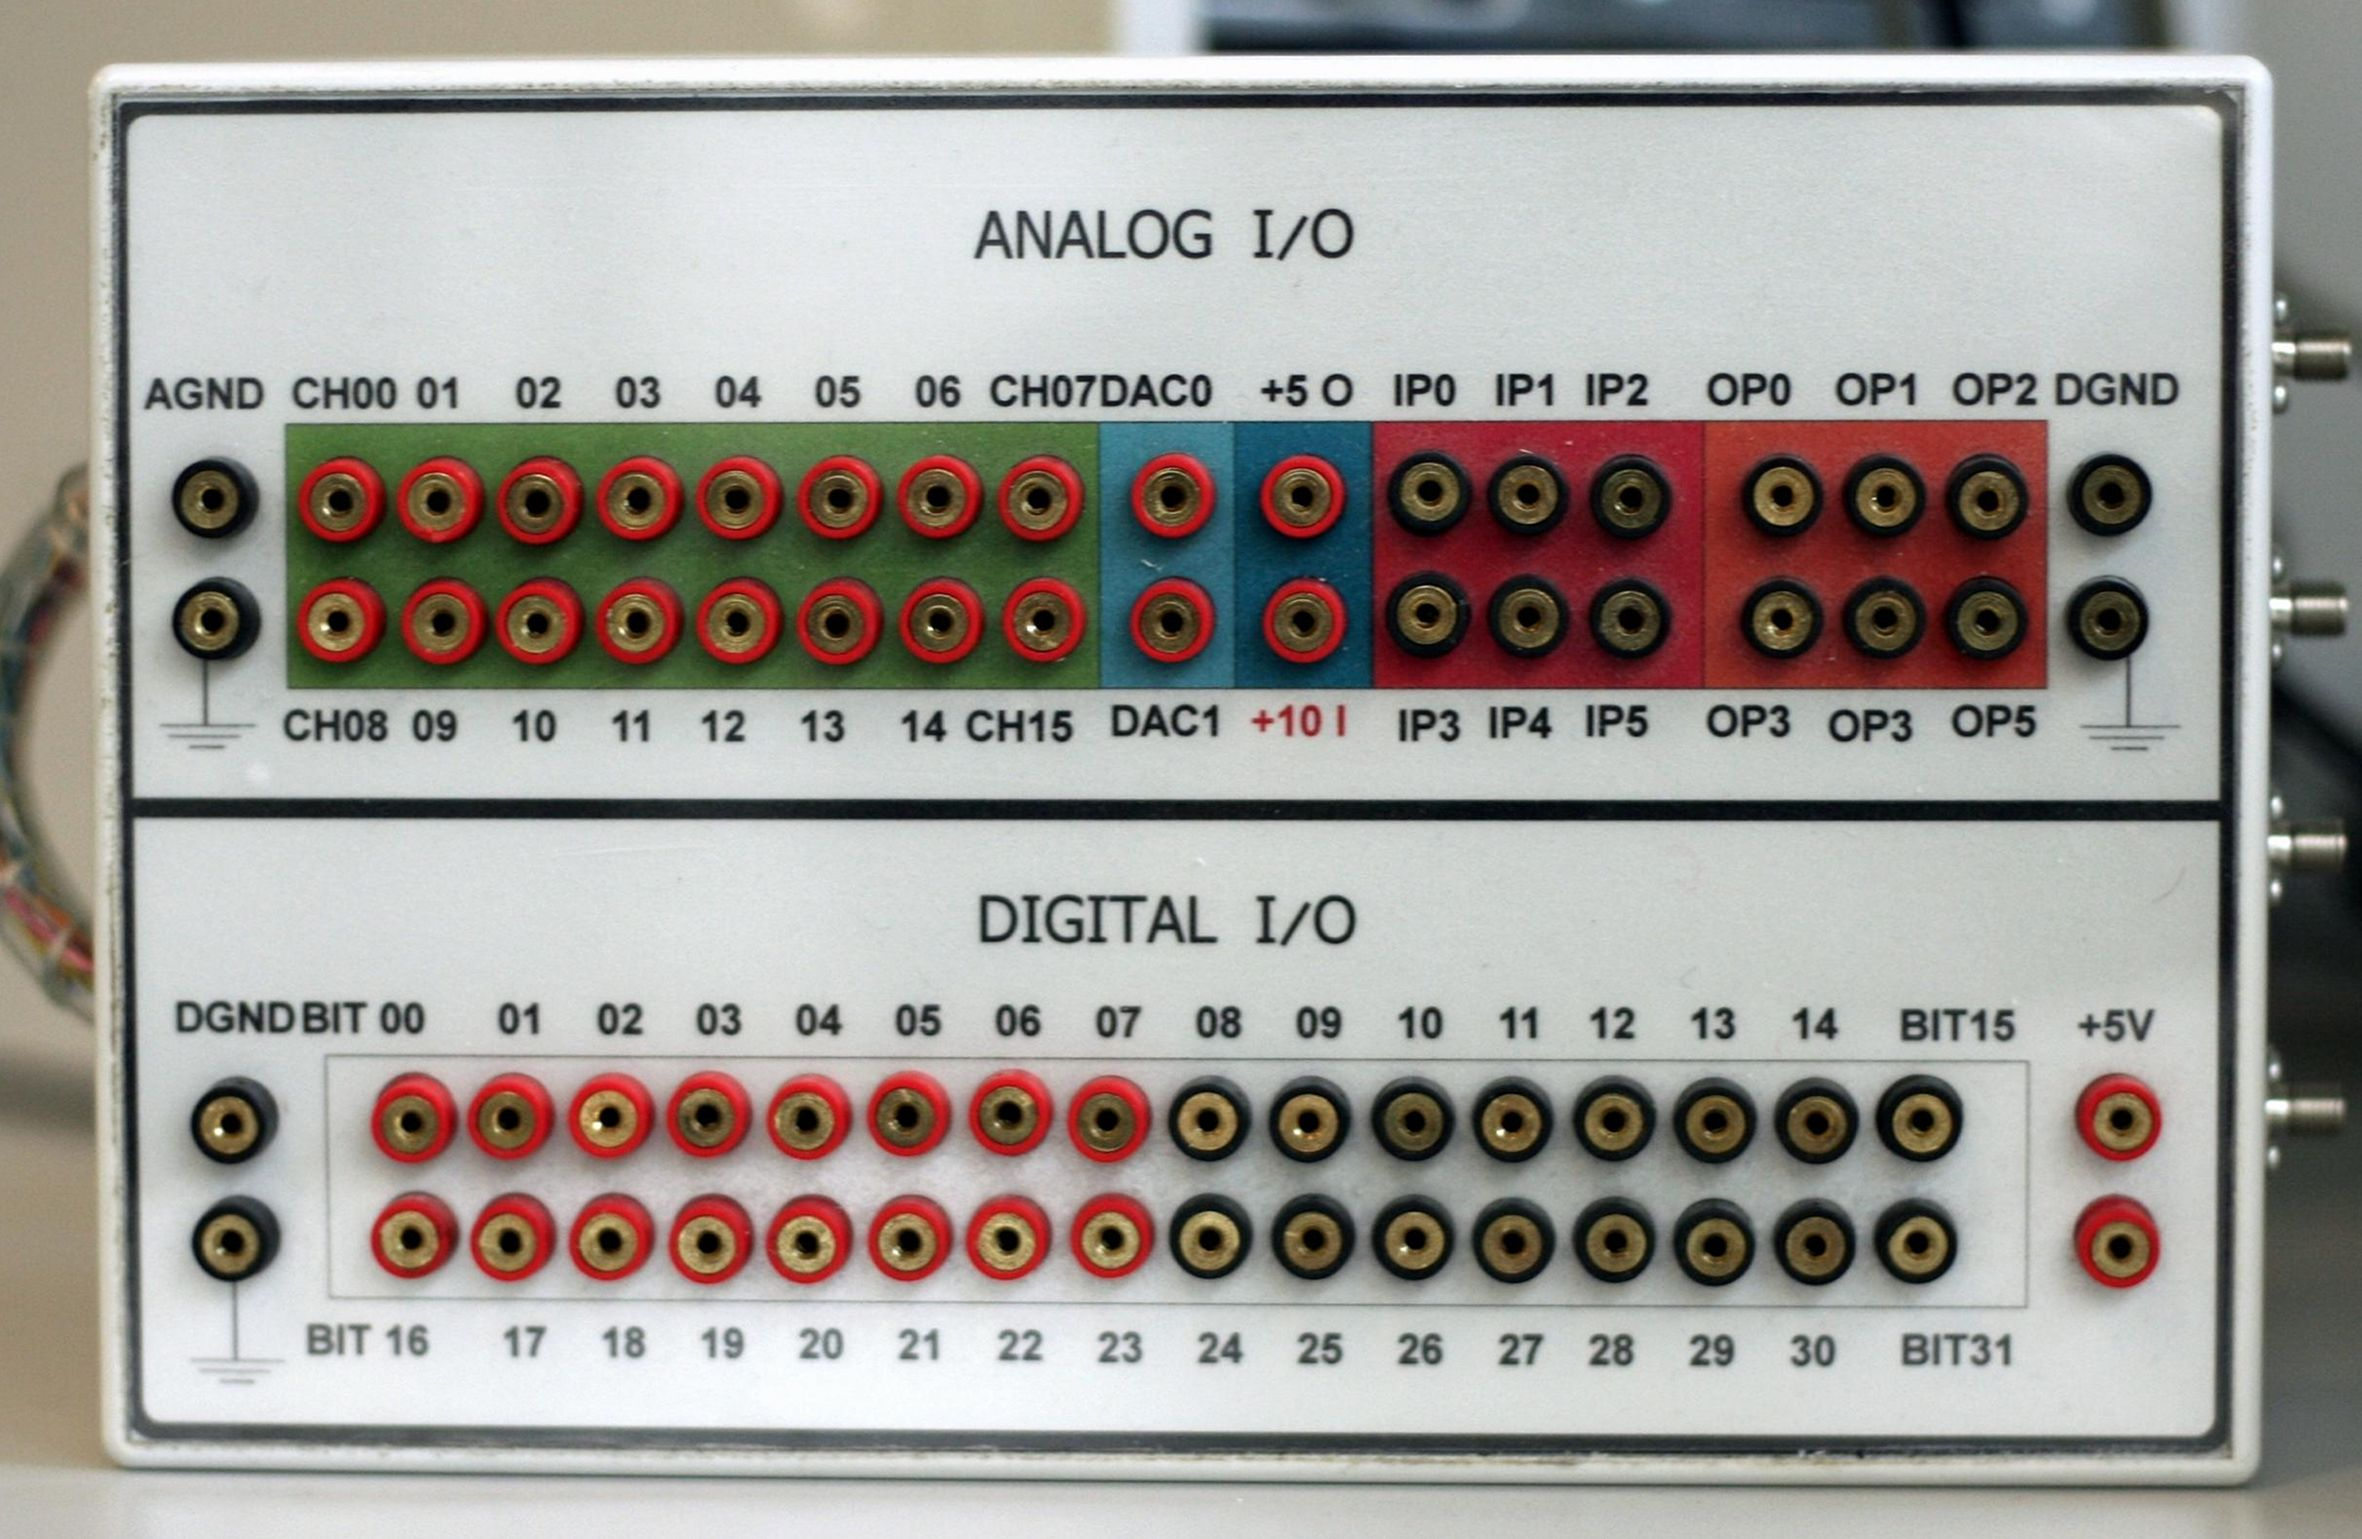
\includegraphics[angle=90]{exterior.jpg}}

\begin{frame}{Caja de conexiones}
    \begin{center}
	\begin{figure}
	    \hspace{\stretch{3}}
	    \begin{minipage}[top][\exterior][c]{.4\textwidth}
		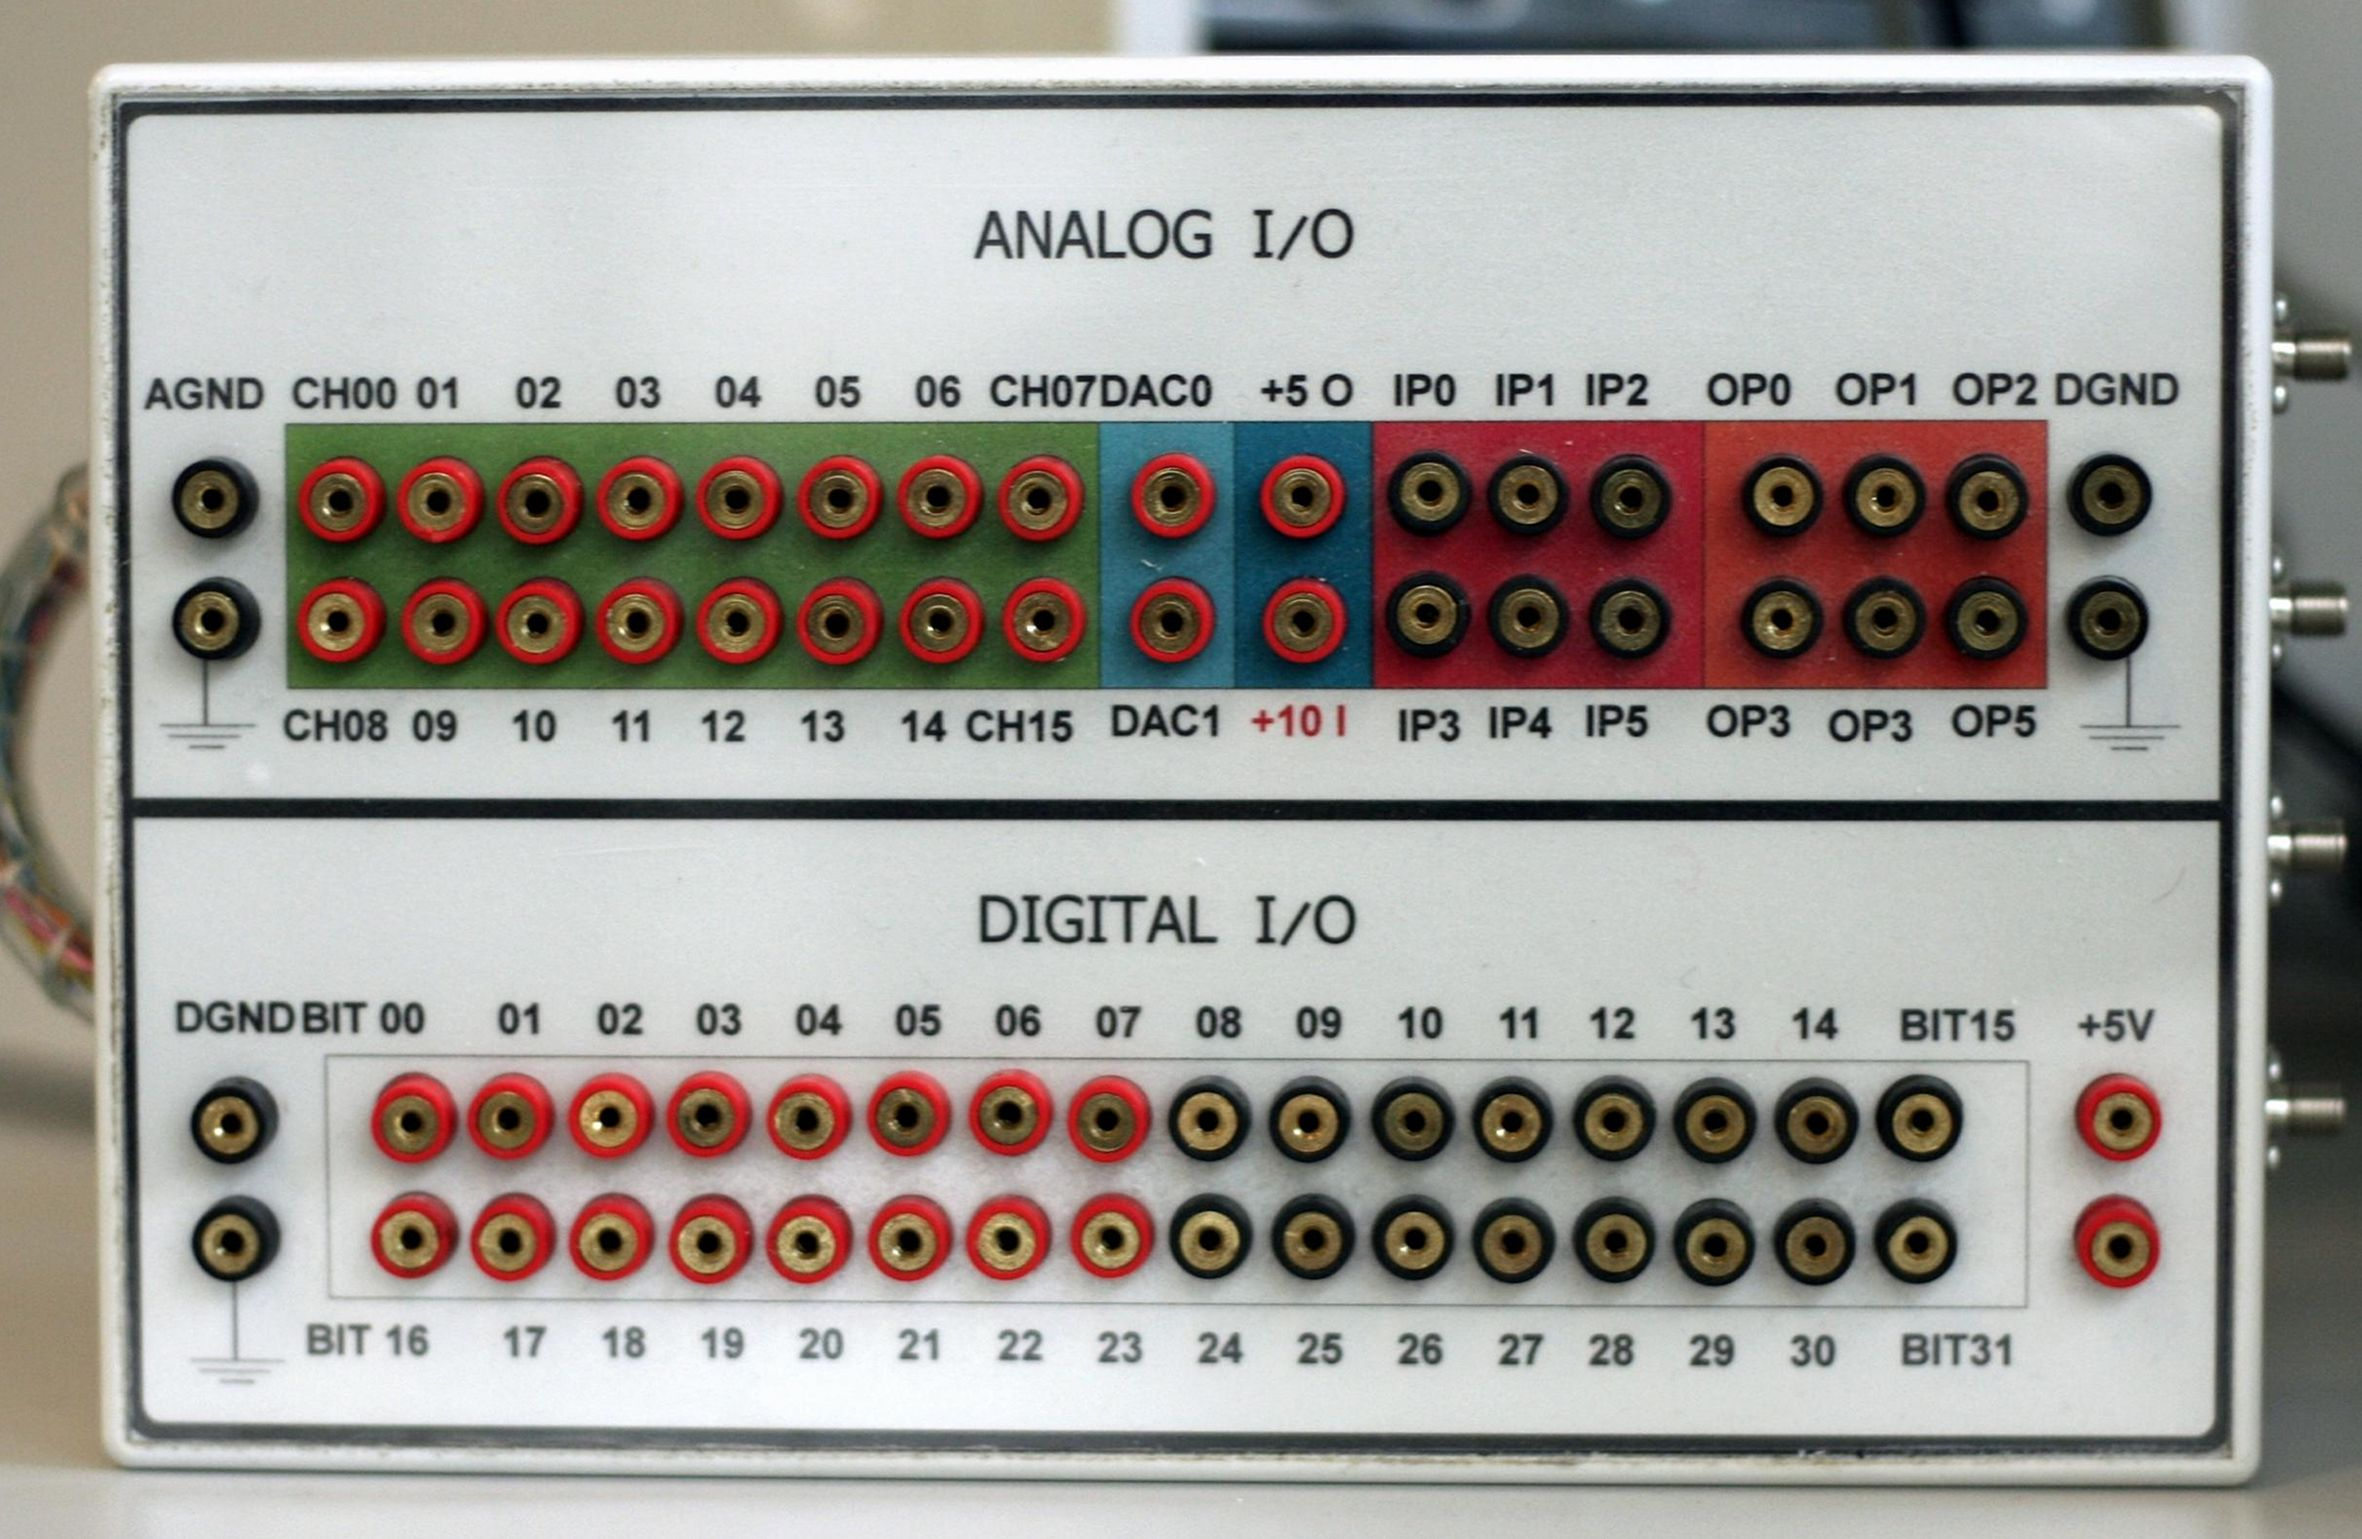
\includegraphics[angle=90]{exterior.jpg}
	    \end{minipage}
	    \hspace{\stretch{.5}}
	    \begin{minipage}[top][\exterior][c]{.4\textwidth}
		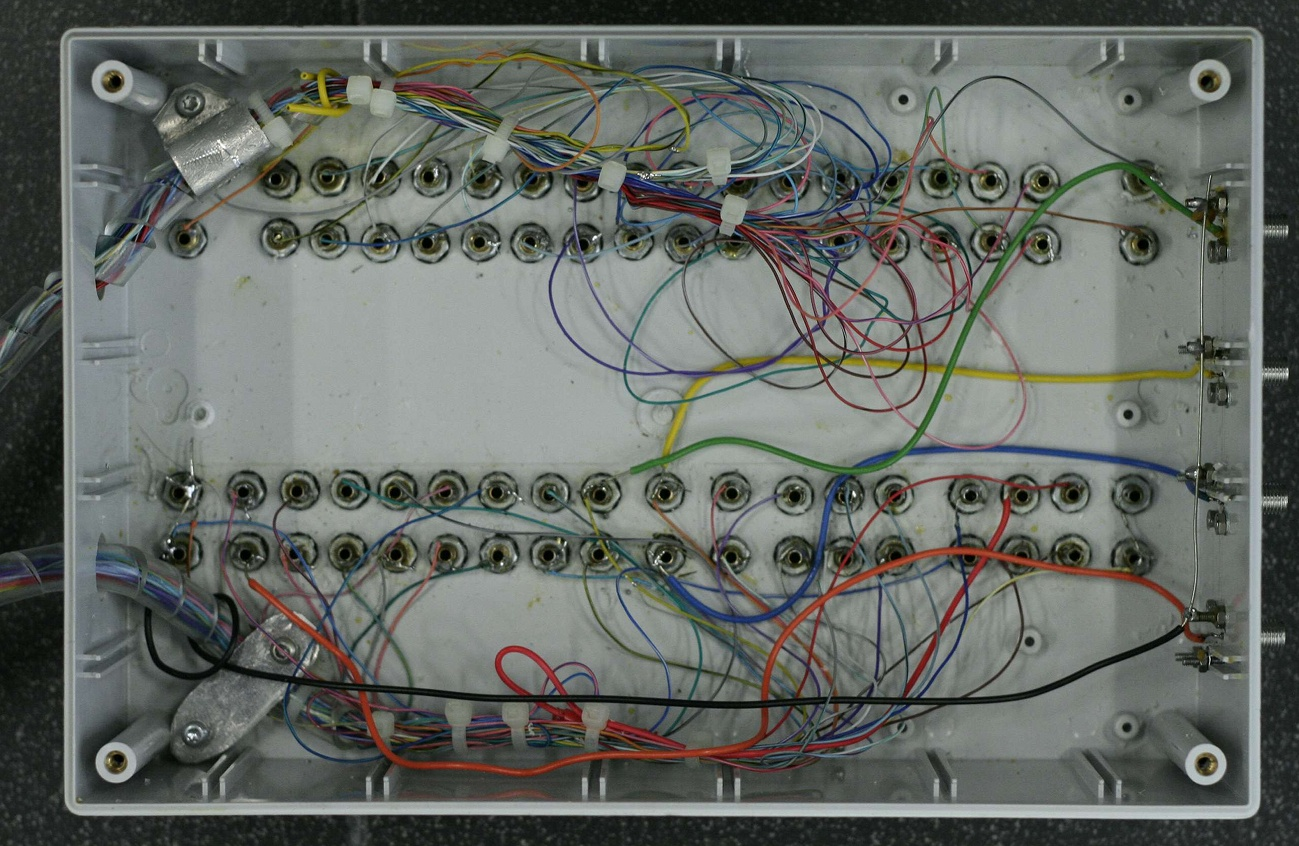
\includegraphics[angle=90]{interior.jpg}
	    \end{minipage}
	    \hspace{\stretch{1}}
	    \caption{Vistas interna y externa de la caja de conexiones}
	    \label{fig:connectionbox}
	\end{figure}
    \end{center}
\end{frame}


\subsection{Capa de control y presentación}

\begin{frame}{Objetivos}
\end{frame}

\begin{frame}{Diseño conceptual}
\end{frame}

\begin{frame}{Diseño conceptual 2}
\end{frame}


\section{Realización de los ensayos}

\subsection{Teoría de los ENDUS}

\begin{frame}{Características de los ultrasonidos}
    \begin{itemize}
	\item Son perturbaciones mecánicas que viajan a través de un medio
	    elástico.
	\item Banda de frecuencia de 20 kHz a 1000 MHz (límite
	    tecnológico).
	\item Banda de frecuencia utilizada en ENDUS de 20 kHz a 25 MHz.
	\item Sus propiedades son invariantes con la frecuencia.
	\item Cuatro tipos de onda ultrasónica: \emph{longitudinales},
	    \emph{transversales}, \emph{de superficie} y \emph{ondas de
	    Lamb}.
    \end{itemize}
\end{frame}

\begin{frame}{Técnicas utilizadas en los ensayos}
\end{frame}

\begin{frame}{Ruido estructural}
\end{frame}


\subsection{Ensayos realizados}

\begin{frame}{Objetivos de las pruebas}
\end{frame}

\begin{frame}{Metodología}
\end{frame}

\begin{frame}{Equipo utilizado}
\end{frame}

\begin{frame}{Resultados y conclusiones}
\end{frame}


\end{document}
